\begin{center}
   \textbf{\titlePageWorkType~№\titlePageWorkNumber~\titlePageWorkPart}
\end{center}

\textbf{Тема}: <<\titlePageTopic>>

\textbf{Цель работы}: 

\begin{enumerate}
   \item Знакомство со структурой файла листинга, получаемого при ассемблировании, структурой машинных команд процессора.
   \item Изучение основных приемов отладки программ и основных возможностей отладчика Turbo Debugger (TD).
\end{enumerate}

\begin{center}
   \textbf{Ход работы}:
\end{center}

\subparagraph{Задание 4.1}

\textbf{Условие}:
\begin{itemize}
   \item Изучить предложенный материал по структуре и назначению полей файла листинга ассемблерной программы. 
   \item Изучить структуру машинной команды.
\end{itemize}

\textbf{Решение}:

\begin{table}[!ht]
   \centering
   \caption{Структура листинга}
   \begin{tabular}{|l|p{1.3cm}|l|p{2cm}|l|l|} 
      \hline
               & 11           & 0003      & 8E D8        & Metka1:   mov   ds, ax   ; установить регистр DS \\ \hline
      глубина  & номер строки & смещение  & машинный код & исходный текст программы                         \\ \hline
   \end{tabular}
\end{table}

\subparagraph{Задание 4.2}

\textbf{Условие}:
Пользуясь информацией лаб.раб.1, написать программу \path{Lab2.asm}, работающую по следующему алгоритму:
\begin{itemize}
   \item вывести на экран первые N символов фамилии студента (использовать функцию 40h DOS INT 21h) – число N задается преподавателем;
   \item вывести строку полностью в цикле N-1 раз на экран. Привести программу в отчете.
\end{itemize}

\textbf{Решение}:

\lstinputlisting[
   name=Lab2.asm,
   language={[x86masm]Assembler},
   tabsize=8,
   basicstyle=\ttfamily\scriptsize,
   numbers=left,
]
{../../src/lab2.asm}

\newpage

\begin{lstlisting}[language=Terminal]
$ C:\tasm\tasm.exe Lab2.asm
\end{lstlisting}
   
\begin{lstlisting}[language=Out]
Turbo Assembler  Version 2.0  Copyright (c) 1988, 1990 Borland International

Assembling file:     Lab2.asm
Error messages:      None
Warning messages:    None
Passes:              1
Remaining memory:    475k
\end{lstlisting}

\begin{lstlisting}[language=Terminal]
$ C:\tasm\tlink.exe LAB2.OBJ
\end{lstlisting}

\begin{lstlisting}[language=Out]
Turbo Link  Version 2.0  Copyright (c) 1987, 1989 Borland International
\end{lstlisting}

\begin{lstlisting}[language=Terminal]
$ LAB2.EXE
\end{lstlisting}

\begin{lstlisting}[language=Out]
Galan
Galanin
Galanin
Galanin
Galanin
\end{lstlisting}

\subparagraph{Задание 4.3}

\textbf{Условие}:
Получить файл листинга и внимательно ознакомиться с его форматом и содержимым.

\textbf{Решение}:

\begin{lstlisting}[language=Terminal]
$ C:\tasm\tasm.exe /l Lab2.asm
\end{lstlisting}

\begin{lstlisting}[language=Out]
Turbo Assembler  Version 2.0  Copyright (c) 1988, 1990 Borland International

Assembling file:   Lab2.asm
Error messages:    None
Warning messages:  None
Passes:            1
Remaining memory:  469k
\end{lstlisting}

\textbf{Создался} объктный файл \textbf{LAB2.OBJ} и файл листинга \textbf{LAB2.LST}.

\begin{figure}[h]
    \centering
    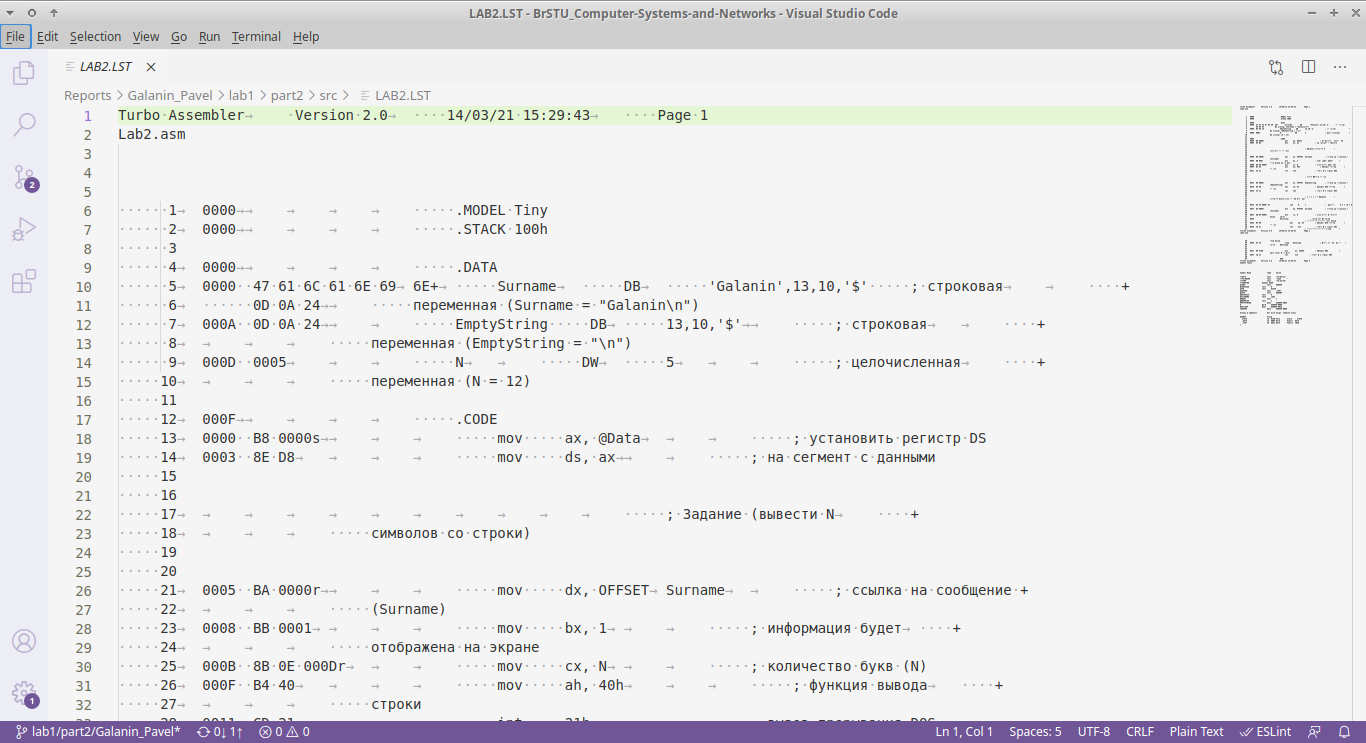
\includegraphics[width=18cm]{../_INCLUDES/lst.png}
    \caption{LAB2.LST в VS Code}
\end{figure}

\subparagraph{Задание 4.4}

\textbf{Условие}:
В любой инструкции с двумя операндами удалить один операнд и проассемблировать программу с получением файла листинга. Какие выходные файлы создаются в этом случае? Что добавляется в листинге? Привести результаты наблюдений в отчете и объяснить их.

\textbf{Решение}:

\begin{lstlisting}[language=Terminal]
$ C:\tasm\tasm.exe Lab2.asm,,Lab2-1.lst
\end{lstlisting}

\begin{lstlisting}[language=Out]
Turbo Assembler  Version 2.0  Copyright (c) 1988, 1990 Borland International

Assembling file:   Lab2.asm
Error messages:    None
Warning messages:  None
Passes:            1
Remaining memory:  469k
\end{lstlisting}

\textbf{Создался} файл листинга \textbf{LAB2-1.LST} и объктный файл \textbf{LAB2.OBJ}.

\begin{lstlisting}[language=Terminal]
$ C:\tasm\tasm.exe Lab2.asm,,Lab2-2.lst
\end{lstlisting}

\begin{lstlisting}[language=Out]
Turbo Assembler  Version 2.0  Copyright (c) 1988, 1990 Borland International

Assembling file:   Lab2.asm
**Error** Lab2.asm(11) Too few operands to instruction
Error messages:    1
Warning messages:  None
Passes:            1
Remaining memory:  469k
\end{lstlisting}

\textbf{Создался} только файл листинга \textbf{LAB2-2.LST} (объектный файл \textbf{LAB2.OBJ не создался}).

\begin{figure}[h]
    \centering
    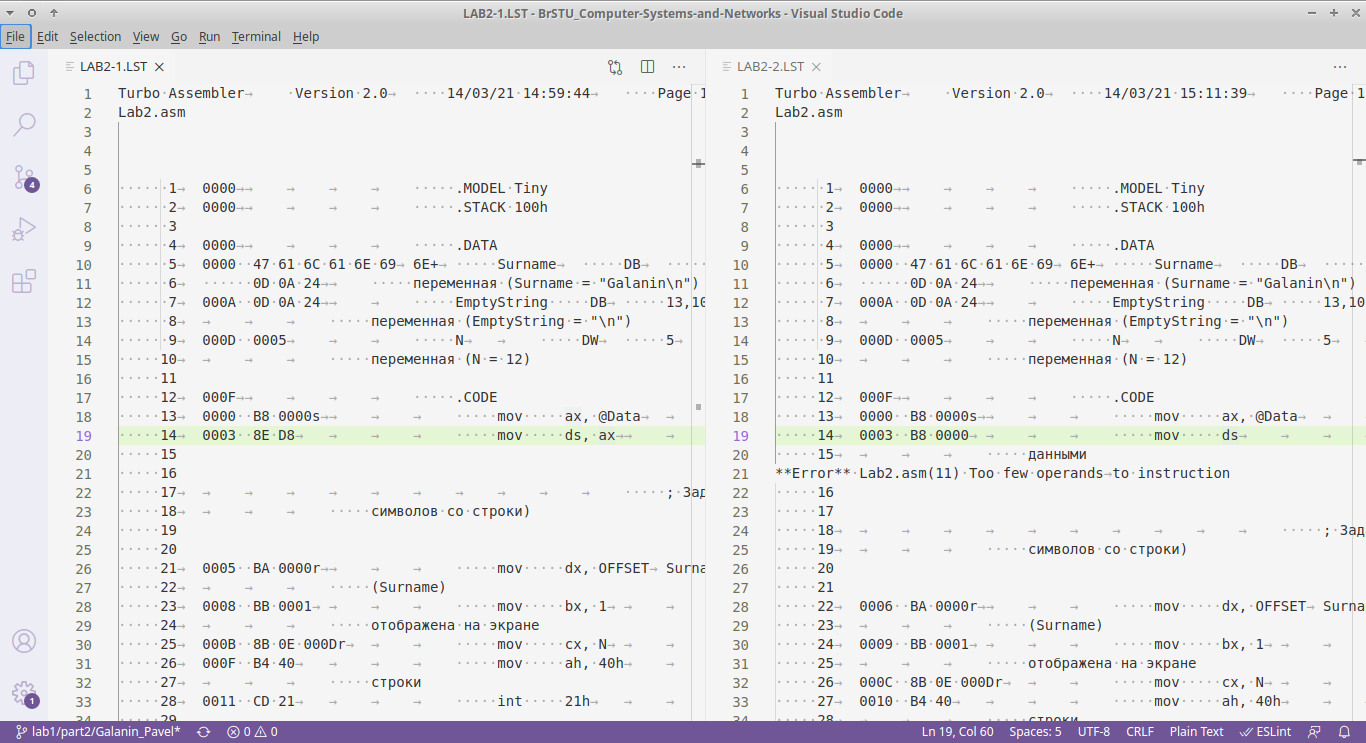
\includegraphics[width=18cm]
        {../_INCLUDES/task-4-4/lst1-and-lst2.png}
    \caption{Сравнение LAB2-1.LST и LAB2-2.LST в VS Code}
\end{figure}

\subparagraph{Задание 4.5}

\textbf{Условие}:
Восстановить исходную программу и создать загрузочный модуль Lab2.exe (при этом использовать команду \textbf{d:\textbackslash\/tasm\textbackslash\/tasm /zi lab2.asm} на этапе трансляции и команду lab2.obj \textbf{d:\textbackslash\/tasm\textbackslash\/tlink /v lab2.obj} на этапе компоновки. Привести в отчете назначение ключей \textbf{/zi} и \textbf{/v}).

\textbf{Решение}:

\begin{lstlisting}[language=Terminal]
$ d:\tasm\tasm /zi lab2.asm
\end{lstlisting}

\begin{lstlisting}[language=Out]
Turbo Assembler  Version 2.0  Copyright (c) 1988, 1990 Borland International

Assembling file:   lab2.asm
Error messages:    None
Warning messages:  None
Passes:            1
Remaining memory:  473k
\end{lstlisting}

Размер объектного файла LAB2.OBJ был \textbf{309 байт}, стал \textbf{577 байт} (в 1.867 раз больше).

\begin{lstlisting}[language=Terminal]
$ d:\tasm\tlink /v lab2.obj
\end{lstlisting}

\begin{lstlisting}[language=Out]
Turbo Link  Version 2.0  Copyright (c) 1987, 1989 Borland International
\end{lstlisting}

Размер исполняемого файла LAB2.EXE был \textbf{597 байт}, стал \textbf{1,32 КБ (1 360 байт)} (в 2.278 раз больше).

Ключ \textbf{/zi} управляет включением в объектный файл номеров строк исходной программы и другой информации, не требуемой при выполнении программы, но используемой отладчиком.

Ключ \textbf{/v} передает в загрузочный файл символьную информацию, позволяющую отладчику TD выводить на экран полный текст исходной программы, включая метки, комментарии и прочее.

\subparagraph{Задание 4.6 (1)}

\textbf{Условие}:
Загрузить программу в отладчик (\textbf{td \path{d:\asm\lab2}}). Какими способами это можно сделать? Отразить способы в отчете.

\textbf{Решение}:

\begin{lstlisting}[language=Terminal]
    $ C:\td\td.exe lab2
\end{lstlisting}

\begin{figure}[!htp]
    \centering
    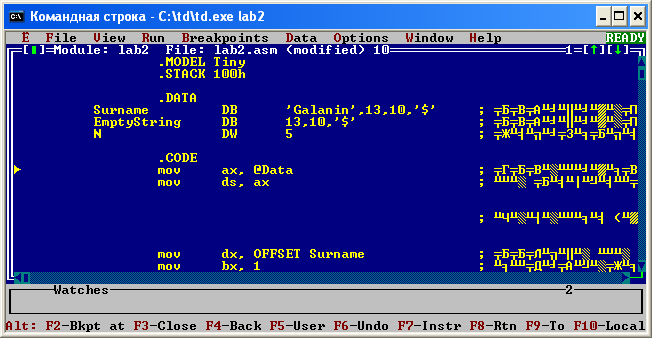
\includegraphics[width=11.2cm]{../_INCLUDES/td.png}
    \caption{td lab2}
\end{figure}

Загрузить программу в отладчик можно:
\begin{enumerate}
    \item Прописав команду \verb|$ td path\to\file|.
    \item В программе Turbo Debugger нажать \textbf{F10}. Нажать \textbf{влево}, выбрав пункт \textbf{File}. Нажать \textbf{Enter}. Выбираем пункт \textbf{Open}.
\end{enumerate}

\begin{figure}[!htp]
    \centering
    \begin{minipage}{0.48\textwidth}
        \centering
        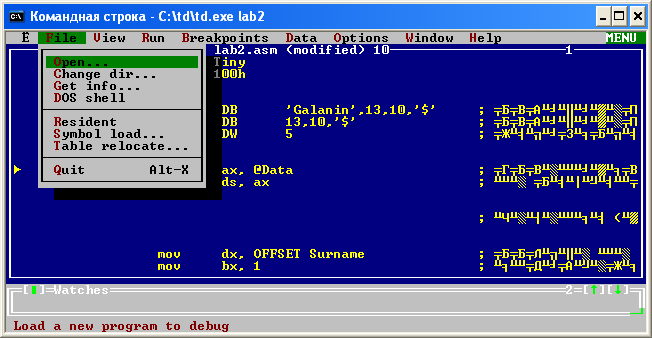
\includegraphics[width=.98\linewidth]
            {../_INCLUDES/task-4-6-1/td-file.png}
        \caption{td >\textbf{FILE}}
    \end{minipage}
    \begin {minipage}{0.48\textwidth}
        \centering
        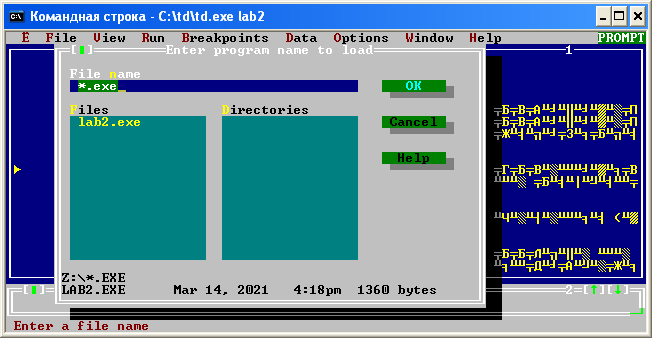
\includegraphics[width=.98\linewidth]
            {../_INCLUDES/task-4-6-1/td-file-open.png}
        \caption{td >\textbf{FILE}>\textbf{OPEN}}
    \end{minipage}
\end{figure}

\subparagraph{Задание 4.6 (2)}

\textbf{Условие}:
Выполнить программу по шагам, нажимая клавишу \textbf{F7}, до конца. Проcмотреть содержимое экрана (\textbf{Alt} + \textbf{F5}). После какой операции ассемблера на экране появляются строки?
 
\textbf{Решение}:

Выполняю программу нажимая клавишу \textbf{F7}.

Просматриваю консоль клавишами \textbf{Alt} + \textbf{F5}.

Далее выполняю программу нажимая клавишу \textbf{F7}.

Просматриваю консоль клавишами \textbf{Alt} + \textbf{F5}.

Далее выполняю программу нажимая клавишу \textbf{F7}.

Просматриваю консоль клавишами \textbf{Alt} + \textbf{F5}.

Так до тех пор пока не пройдем команду \textbf{int 21h}: вызовится прерывание DOS и появится вывод в консоль.

Turbo Debugger по нажатию \textbf{F7} на рисунке \ref{fig:task_4_6_2__F7} (стр. \pageref{fig:task_4_6_2__F7}).

Turbo Debugger по нажатию \textbf{Alt} + \textbf{F5} на рисунке \ref{fig:task_4_6_2__Alt_F5} (стр. \pageref{fig:task_4_6_2__Alt_F5}).

\begin{figure}[!htp]
    \centering
    \begin{minipage}{0.48\textwidth}
        \centering
        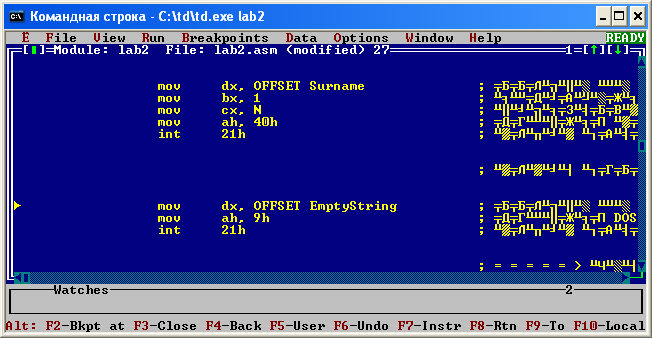
\includegraphics[width=.98\linewidth]
            {../_INCLUDES/task-4-6-2/F7.png}
        \caption{Нажимаю \textbf{F7}\\в Turbo Debugger}
        \label{fig:task_4_6_2__F7}
    \end{minipage}
    \begin {minipage}{0.48\textwidth}
        \centering
        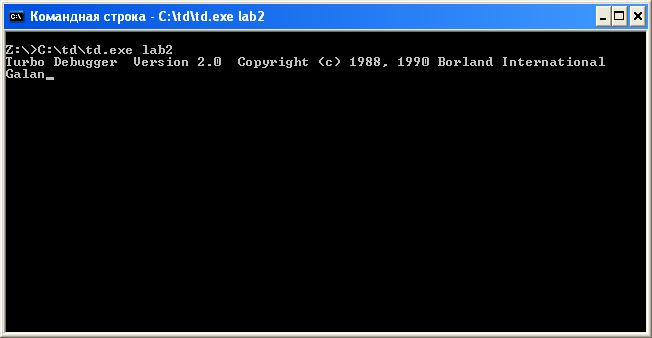
\includegraphics[width=.98\linewidth]
            {../_INCLUDES/task-4-6-2/Alt+F5.png}
        \caption{Нажимаю \textbf{Alt} + \textbf{F5}\\в Turbo Debugger}
        \label{fig:task_4_6_2__Alt_F5}
    \end{minipage}
\end{figure}

\subparagraph{Задание 4.7}

\textbf{Условие}:
Вывести в окне Watch (View->Watch) содержимое выходного буфера. 

\textbf{Решение}:

Жмем \textbf{F10}. Жмем два раза \textbf{влево}. \textbf{Enter}. Жмем три раза \textbf{вниз}. \textbf{Enter}.
Рисунок~\ref{fig:task_4_7__menu_watches} (стр.~\pageref{fig:task_4_7__menu_watches}).

Вводим watch, например, 21h. Нажимаем ОК (\textbf{Enter}).
Рисунок~\ref{fig:task_4_7__watches_21h} (стр.~\pageref{fig:task_4_7__watches_21h}).

Результат на рисунке~\ref{fig:task_4_7__watches_result} (стр.~\pageref{fig:task_4_7__watches_result}).

\begin{figure}[!htp]
    \centering
    \begin{minipage}{0.32\textwidth}
        \centering
        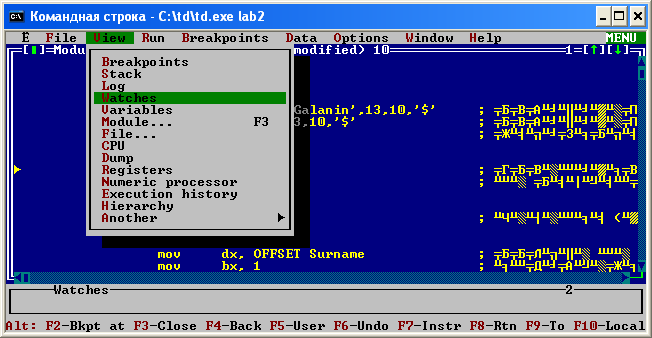
\includegraphics[width=.99\linewidth]
            {../_INCLUDES/task-4-7/td-view-watches.png}
        \caption{>\textbf{View}>\textbf{Wathes}}
        \label{fig:task_4_7__menu_watches}
    \end{minipage}
    \begin {minipage}{0.32\textwidth}
        \centering
        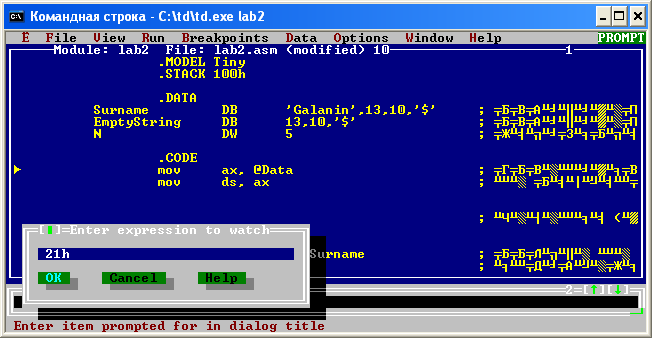
\includegraphics[width=.99\linewidth]
            {../_INCLUDES/task-4-7/watch-21h.png}
        \caption{Пишем watch}
        \label{fig:task_4_7__watches_21h}
    \end{minipage}
    \begin {minipage}{0.32\textwidth}
        \centering
        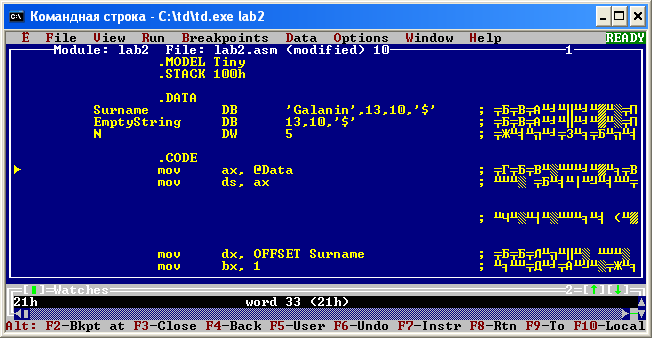
\includegraphics[width=.99\linewidth]
            {../_INCLUDES/task-4-7/watch-result.png}
        \caption{Результат watch}
        \label{fig:task_4_7__watches_result}
    \end{minipage}
\end{figure}

\subparagraph{Задание 4.8}

\textbf{Условие}:
Выполнить программу (Goto cursor - клавиша \textbf{F4}) до места начала цикла. 

\textbf{Решение}:

Есть стрелка.
Рисунок~\ref{fig:task_4_8__1} (стр.~\pageref{fig:task_4_8__1}).
Нижние подчеркивание двигается.
Рисунок~\ref{fig:task_4_8__2} (стр.~\pageref{fig:task_4_8__2}).
Жмем \textbf{F4}. Стрелка встала на нижнее подчеркивание.
Рисунок~\ref{fig:task_4_8__3} (стр.~\pageref{fig:task_4_8__3}).

\begin{figure}[!htp]
    \centering
    \begin{minipage}{0.32\textwidth}
        \centering
        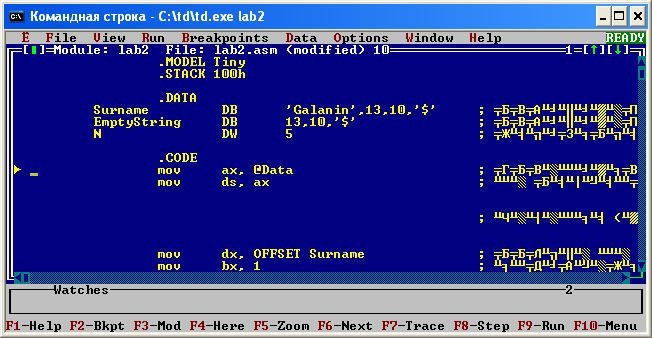
\includegraphics[width=.99\linewidth]
            {../_INCLUDES/task-4-8/1.png}
        \caption{1) Начальное состояние}
        \label{fig:task_4_8__1}
    \end{minipage}
    \begin {minipage}{0.32\textwidth}
        \centering
        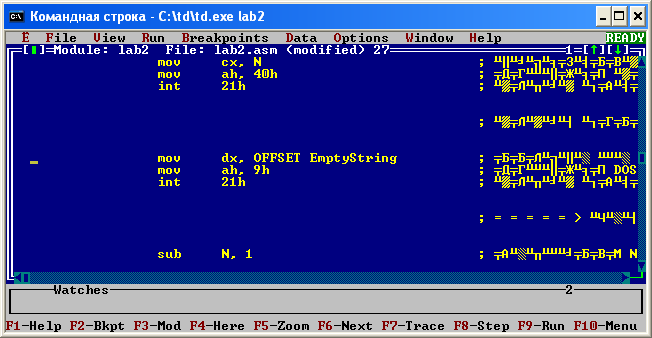
\includegraphics[width=.99\linewidth]
            {../_INCLUDES/task-4-8/2.png}
        \caption{2) Поставили метку стрелками \textbf{вверх}-\textbf{вниз}}
        \label{fig:task_4_8__2}
    \end{minipage}
    \begin {minipage}{0.32\textwidth}
        \centering
        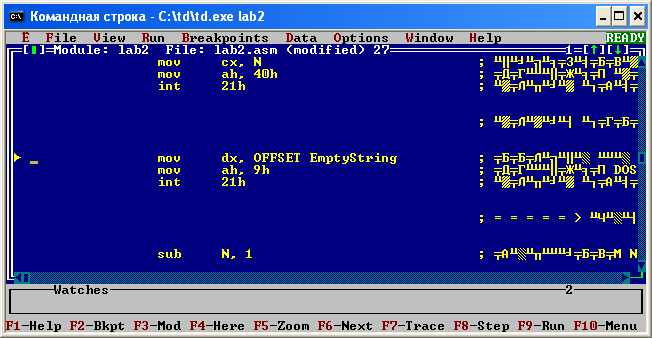
\includegraphics[width=.99\linewidth]
            {../_INCLUDES/task-4-8/3.png}
        \caption{3) Перешли к метке клавишей \textbf{F4}}
        \label{fig:task_4_8__3}
    \end{minipage}
\end{figure}

\subparagraph{Задание 4.9}

\textbf{Условие}:
Выполнить 2 прохода цикла по F7, контролируя значения регистров. Для этого необходимо открыть окно CPU (View->CPU). Какие регистры изменяются в цикле?

Привести результаты выполнения данного фрагмента программы в отчете в виде таблицы: пример таблица~\ref{tab:task_4_9} (стр.~\pageref{tab:task_4_9}).

\begin{table}[!ht]
    \centering
    \caption{Пример таблицы для задания}
    \label{tab:task_4_9}
    \begin{tabular}{|c|c|c|c|c|c|} 
        \hline
        № шага  & IP  & AX  & BX  & CX  & DX  \\ \hline
        \hline
        1       &     &     &     &     &     \\ \hline
        2       &     &     &     &     &     \\ \hline
        ...     &     &     &     &     &     \\ \hline
    \end{tabular}
\end{table}

Объяснить в отчете изменения регистров

\textbf{Решение}:

В Turbo Debugger жмем F10. Попадаем в Меню. Жмем два раза вправо. Выбираем пунтк View. Enter. Жмем 7 раз вниз. Enter. Вводим для поиска метку NextLoop. Рисунок~\ref{fig:task_4_9__View_Watches} (стр.~\pageref{fig:task_4_9__View_Watches}).

Жмем Alt+F9. Вводим NextLoop. Enter. Рисунок~\ref{fig:task_4_9__Alt_F9} (стр.~\pageref{fig:task_4_9__Alt_F9}).

Перешли к метке. Результат на рисуноке~\ref{fig:task_4_9__Alt_F9_result} (стр.~\pageref{fig:task_4_9__Alt_F9_result}).

\begin{figure}[!htp]
    \centering
    \begin{minipage}{0.32\textwidth}
        \centering
        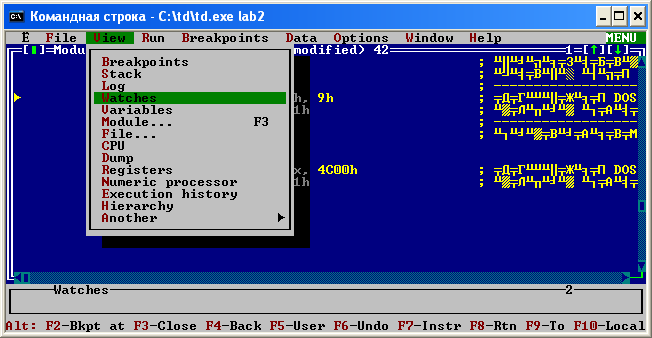
\includegraphics[width=.99\linewidth]
            {../_INCLUDES/task-4-9/td-View-Watches.png}
        \caption{\textbf{View}>\textbf{Wathes}}
        \label{fig:task_4_9__View_Watches}
    \end{minipage}
    \begin {minipage}{0.32\textwidth}
        \centering
        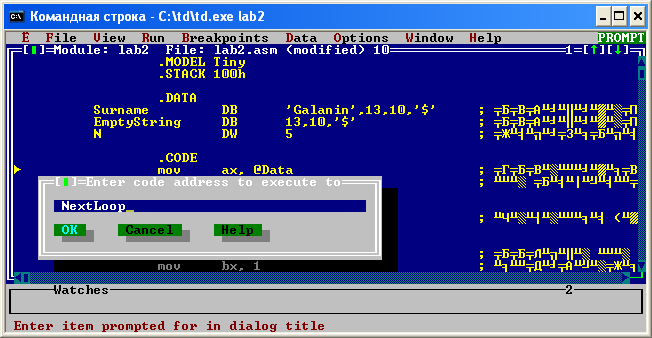
\includegraphics[width=.99\linewidth]
            {../_INCLUDES/task-4-9/td-Alt-F9.png}
        \caption{\textbf{Alt} + \textbf{F9}}
        \label{fig:task_4_9__Alt_F9}
    \end{minipage}
    \begin {minipage}{0.32\textwidth}
        \centering
        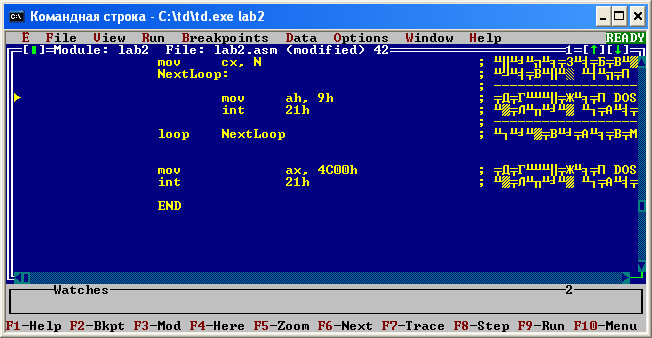
\includegraphics[width=.99\linewidth]
            {../_INCLUDES/task-4-9/td-Alt-F9-result.png}
        \caption{Переход к метке}
        \label{fig:task_4_9__Alt_F9_result}
    \end{minipage}
\end{figure}

Жмем \textbf{F10}. Жмем два раз \textbf{вправо}. Выбираем пункт \textbf{View}. Жмем 7 раз \textbf{вниз}. Выбираем пунт \textbf{CPU}. \textbf{Enter}. Результат на рисуноке~\ref{fig:task_4_9__td_View_CPU} (стр.~\pageref{fig:task_4_9__td_View_CPU}).

\begin{figure}[!htp]
    \centering
    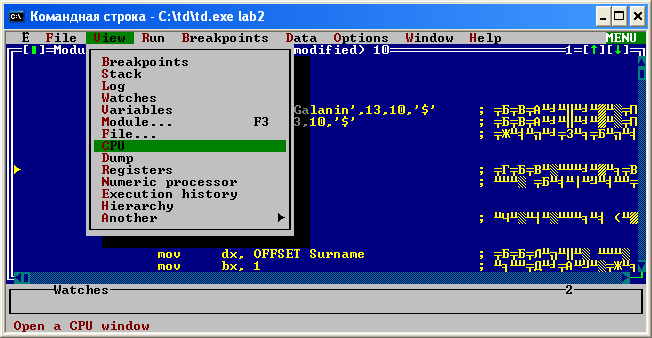
\includegraphics[width=8cm]
        {../_INCLUDES/task-4-9/td-View-CPU.png}
    \caption{}
    \label{fig:task_4_9__td_View_CPU}
\end{figure}

\begin{figure}[!htp]
    \centering
    \begin{minipage}{0.32\textwidth}
        \centering
        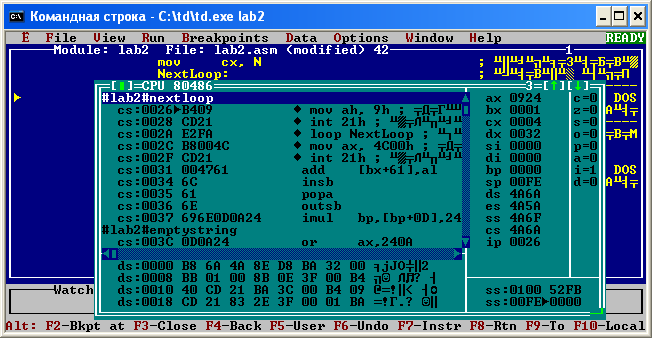
\includegraphics[width=.99\linewidth]
            {../_INCLUDES/task-4-9/0.png}
        \caption{0 Шаг}
        \label{fig:task_4_9}
    \end{minipage}
    \begin {minipage}{0.32\textwidth}
        \centering
        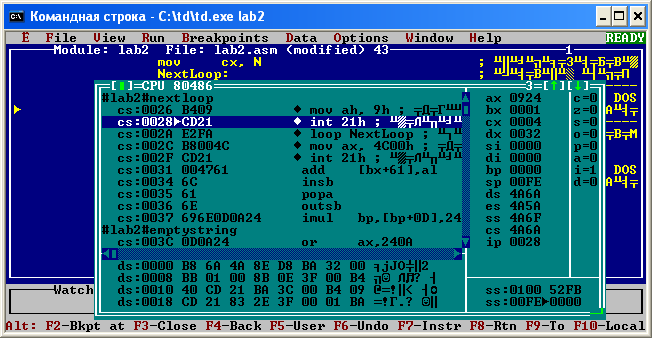
\includegraphics[width=.99\linewidth]
            {../_INCLUDES/task-4-9/1.png}
        \caption{1) \textbf{F7}}
        \label{fig:task_4_9}
    \end{minipage}
    \begin {minipage}{0.32\textwidth}
        \centering
        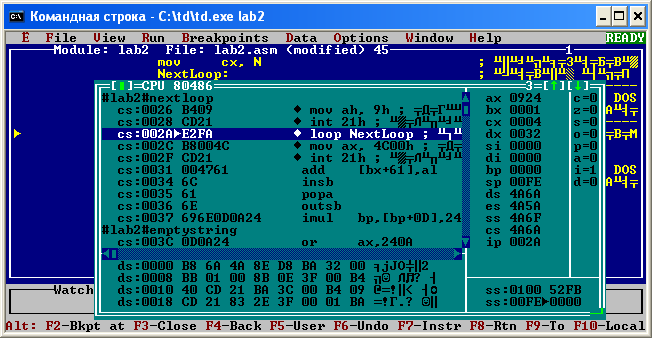
\includegraphics[width=.99\linewidth]
            {../_INCLUDES/task-4-9/2.png}
        \caption{2) \textbf{F7}}
        \label{fig:task_4_9}
    \end{minipage}
\end{figure}

\begin{figure}[!htp]
    \centering
    \begin{minipage}{0.32\textwidth}
        \centering
        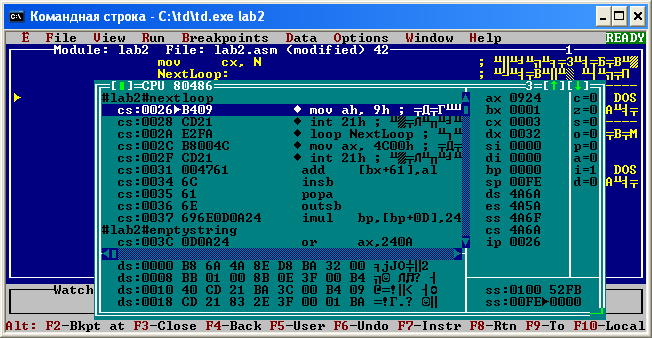
\includegraphics[width=.99\linewidth]
            {../_INCLUDES/task-4-9/3.png}
        \caption{3) \textbf{F7}}
        \label{fig:task_4_9}
    \end{minipage}
    \begin {minipage}{0.32\textwidth}
        \centering
        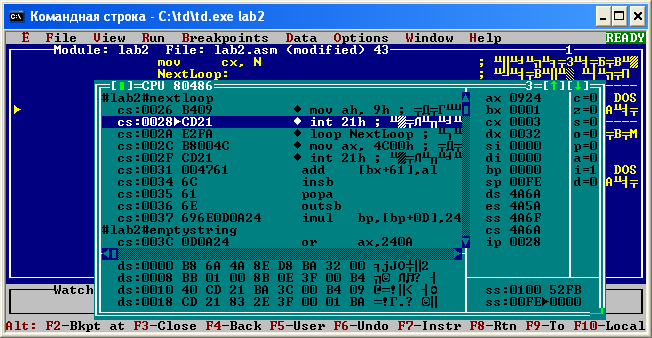
\includegraphics[width=.99\linewidth]
            {../_INCLUDES/task-4-9/4.png}
        \caption{4) \textbf{F7}}
        \label{fig:task_4_9}
    \end{minipage}
    \begin {minipage}{0.32\textwidth}
        \centering
        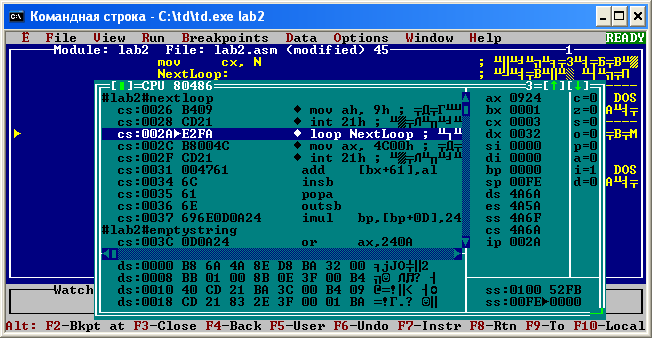
\includegraphics[width=.99\linewidth]
            {../_INCLUDES/task-4-9/5.png}
        \caption{5) \textbf{F7}}
        \label{fig:task_4_9}
    \end{minipage}
\end{figure}

\begin{figure}[!htp]
    \centering
    \begin{minipage}{0.32\textwidth}
        \centering
        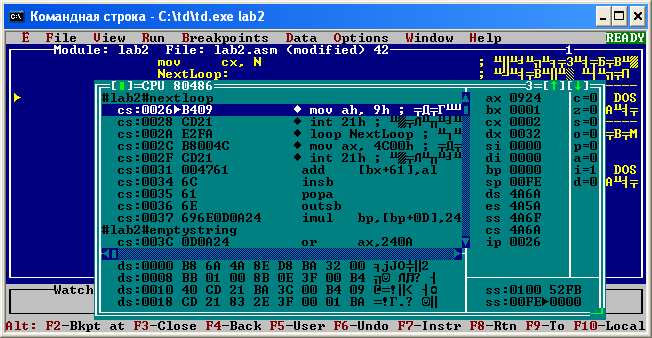
\includegraphics[width=.99\linewidth]
            {../_INCLUDES/task-4-9/6.png}
        \caption{6) \textbf{F7}}
        \label{fig:task_4_9}
    \end{minipage}
    \begin {minipage}{0.32\textwidth}
        \centering
        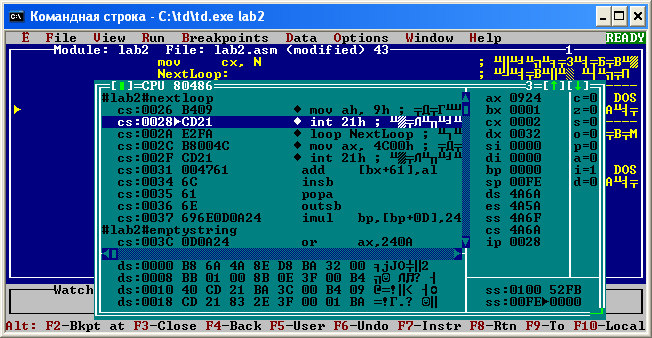
\includegraphics[width=.99\linewidth]
            {../_INCLUDES/task-4-9/7.png}
        \caption{7) \textbf{F7}}
        \label{fig:task_4_9}
    \end{minipage}
    \begin {minipage}{0.32\textwidth}
        \centering
        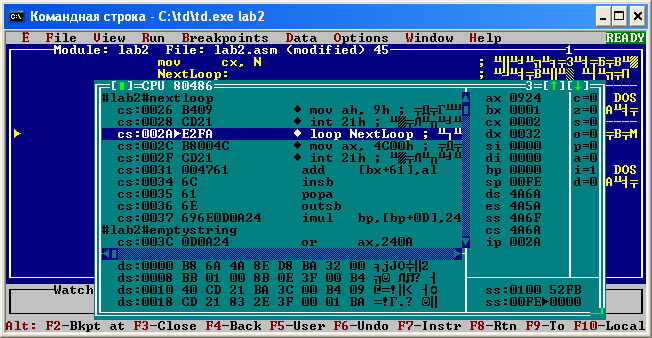
\includegraphics[width=.99\linewidth]
            {../_INCLUDES/task-4-9/8.png}
        \caption{8) \textbf{F7}}
        \label{fig:task_4_9}
    \end{minipage}
\end{figure}

\begin{figure}[!htp]
    \centering
    \begin{minipage}{0.32\textwidth}
        \centering
        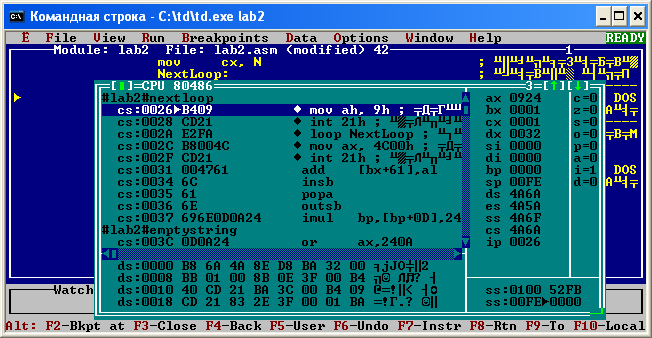
\includegraphics[width=.99\linewidth]
            {../_INCLUDES/task-4-9/9.png}
        \caption{9) \textbf{F7}}
        \label{fig:task_4_9}
    \end{minipage}
    \begin {minipage}{0.32\textwidth}
        \centering
        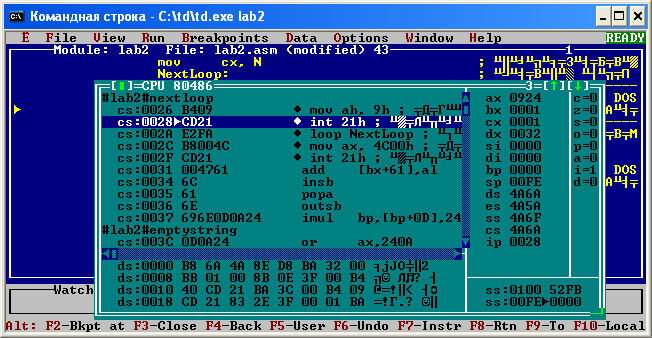
\includegraphics[width=.99\linewidth]
            {../_INCLUDES/task-4-9/10.png}
        \caption{10) \textbf{F7}}
        \label{fig:task_4_9}
    \end{minipage}
    \begin {minipage}{0.32\textwidth}
        \centering
        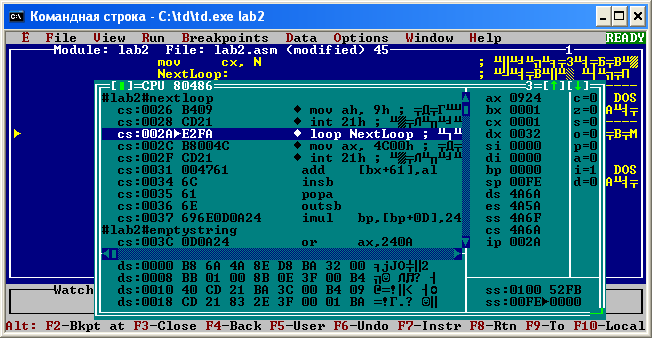
\includegraphics[width=.99\linewidth]
            {../_INCLUDES/task-4-9/11.png}
        \caption{11) \textbf{F7}}
        \label{fig:task_4_9}
    \end{minipage}
\end{figure}

\begin{figure}[!htp]
    \centering
    \begin{minipage}{0.32\textwidth}
        \centering
        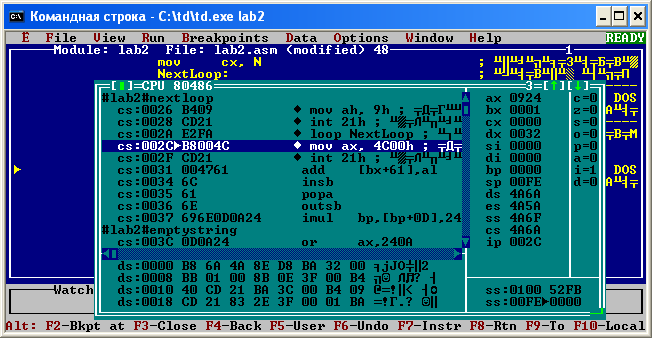
\includegraphics[width=.99\linewidth]
            {../_INCLUDES/task-4-9/12.png}
        \caption{12) \textbf{F7}}
        \label{fig:task_4_9}
    \end{minipage}
    \begin {minipage}{0.32\textwidth}
        \centering
        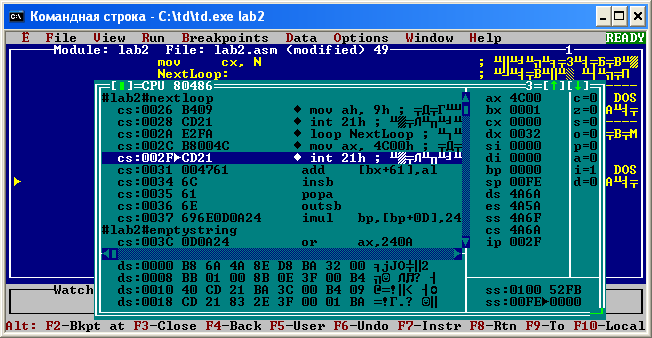
\includegraphics[width=.99\linewidth]
            {../_INCLUDES/task-4-9/13.png}
        \caption{13) \textbf{F7}}
        \label{fig:task_4_9}
    \end{minipage}
    \begin {minipage}{0.32\textwidth}
        \centering
        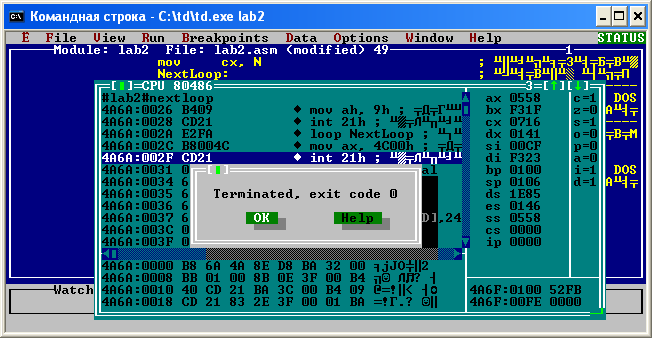
\includegraphics[width=.99\linewidth]
            {../_INCLUDES/task-4-9/14.png}
        \caption{14) \textbf{F7}}
        \label{fig:task_4_9}
    \end{minipage}
\end{figure}

Значение регистров после метки NextLoop с шагом \textbf{F7} в таблице~\ref{tab:task_4_9__table} (стр. \pageref{tab:task_4_9__table}).

\begin{table}[!htp]
    \centering
    \caption{Значения регистров после метки NextLoop с шагом \textbf{F7}}
    \label{tab:task_4_9__table}
    \begin{tabular}{|c|c|c|c|c|c|} 
        \hline
        № шага  & IP    & AX    & BX    & CX    & DX    \\ \hline
        \hline
        0       & 0026  & 0924  & 0001  & 0004  & 0032  \\ \hline
        1       & 0028  & 0924  & 0001  & 0004  & 0032  \\ \hline
        2       & 002A  & 0924  & 0001  & 0004  & 0032  \\ \hline
        3       & 0026  & 0924  & 0001  & 0003  & 0032  \\ \hline
        4       & 0028  & 0924  & 0001  & 0003  & 0032  \\ \hline
        5       & 002A  & 0924  & 0001  & 0003  & 0032  \\ \hline
        6       & 0026  & 0924  & 0001  & 0002  & 0032  \\ \hline
        7       & 0028  & 0924  & 0001  & 0002  & 0032  \\ \hline
        8       & 002A  & 0924  & 0001  & 0002  & 0032  \\ \hline
        9       & 0026  & 0924  & 0001  & 0001  & 0032  \\ \hline
        10      & 0028  & 0924  & 0001  & 0001  & 0032  \\ \hline
        11      & 002A  & 0924  & 0001  & 0001  & 0032  \\ \hline
        12      & 002C  & 0924  & 0001  & 0000  & 0032  \\ \hline
        13      & 002F  & 4c00  & 0001  & 0000  & 0032  \\ \hline
        14      & 0000  & 0558  & F31F  & 0716  & 0141  \\ \hline
    \end{tabular}
\end{table}

\newpage

\subparagraph{Задание 4.10}

\textbf{Условие}:
Остальные проходы цикла выполнить по F8. В чем разница? \textbf{Привести объяснения в отчете.}

\textbf{Решение}:

\textbf{F7} проходит цикл \textbf{cx, N} раз. \textbf{F8} проходит цикл за один раз.

У меня \textbf{F8} метку NextLoop проходит также как и \textbf{F7}. Жму \textbf{F8} 27 раз до конца программы. \textbf{F7} жму 27 раз до конца программы.

\subparagraph{Задание 4.12}

\textbf{Условие}: Вывести содержимое выходного буфера в окне Watches. 

\textbf{Решение}:

В Turbo Debugger захожу в меню клавишей \textbf{F10}. Два раза перемещаюсь \textbf{вправо}. Выбираю вкладку \textbf{View}. \textbf{Enter}. Два раза перемещаюсь \textbf{вниз}. Выбираю вкладку \textbf{Watches}. \textbf{Enter}.
Рисунок~\ref{fig:task_4_12__1} (стр.~\pageref{fig:task_4_12__1}).
Ввожу c клавиатуры \textbf{cx}.
Рисунок~\ref{fig:task_4_12__2} (стр.~\pageref{fig:task_4_12__2}).
Видим снизу в Watches коробке \textbf{cx word 38136 (94F8h)}.
Рисунок~\ref{fig:task_4_12__3} (стр.~\pageref{fig:task_4_12__3}).

\begin{figure}[!htp]
    \centering
    \begin{minipage}{0.32\textwidth}
        \centering
        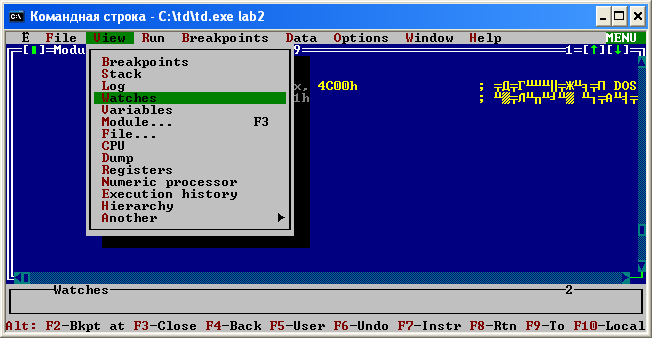
\includegraphics[width=.99\linewidth]
            {../_INCLUDES/task-4-12/1.png}
        \caption{1) \textbf{Watches}}
        \label{fig:task_4_12__1}
    \end{minipage}
    \begin {minipage}{0.32\textwidth}
        \centering
        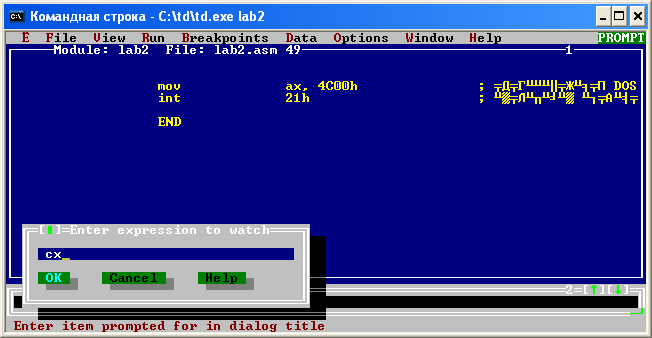
\includegraphics[width=.99\linewidth]
            {../_INCLUDES/task-4-12/2.png}
        \caption{2) Вводим \textbf{cx}}
        \label{fig:task_4_12__2}
    \end{minipage}
    \begin {minipage}{0.32\textwidth}
        \centering
        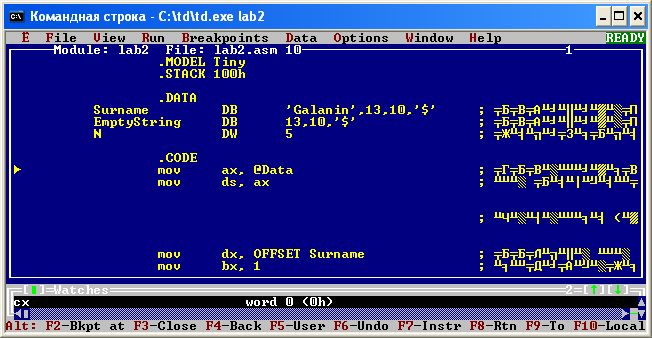
\includegraphics[width=.99\linewidth]
            {../_INCLUDES/task-4-12/3.png}
        \caption{3) Результат}
        \label{fig:task_4_12__3}
    \end{minipage}
\end{figure}


\subparagraph{Задание 4.13 (1)}

\textbf{Условие}: Вывести содержимое регистра CX буфера в окне Watches в шестнадцатеричном формате (Options->Display options->Hex).

\textbf{Решение}:



\subparagraph{Задание 4.13 (2)}

\textbf{Условие}:
Вывести содержимое регистра CX буфера в окне Watches в десятичном формате (Options->Display options->Decimal).

\textbf{Решение}:



\subparagraph{Задание 4.14}

\textbf{Условие}:
Изменить содержимое регистра CX на величину, меньшую на 2 единицы (Data->Evaluate/Modify->Expression=cx, New Value=cx-2). Выполнить пошагово (F7) программу до конца. Что изменилось? Объяснить в отчете.

\textbf{Решение}:



\subparagraph{Задание 4.15}

\textbf{Условие}:
Выполнить команду Animate из меню Run с задержкой 1000 мс.

\textbf{Решение}:



\subparagraph{Задание 4.16}

\textbf{Условие}:
Сбросить программу по Ctrl-F2. Выполнить первые 2 инструкции. Отменить их действие по Alt-F4. Привести объяснения о результате в отчете.

\textbf{Решение}:



\subparagraph{Задание 4.17 (1)}

\textbf{Условие}:
По шагам пройти до первой после int 21h инструкции. Попытаться по Alt-F4 все отменить. Что получилось? Привести объяснения о результате в отчете.

\textbf{Решение}:



\subparagraph{Задание 4.17 (2)}

\textbf{Условие}:
Сбросить программу по Ctrl-F2. По F7 выполнить первые 6 инструкций. Открыть окно Execution History. Отменить последние 3 шага.

\textbf{Решение}:


